\begin{figure}[t]
\centering       
    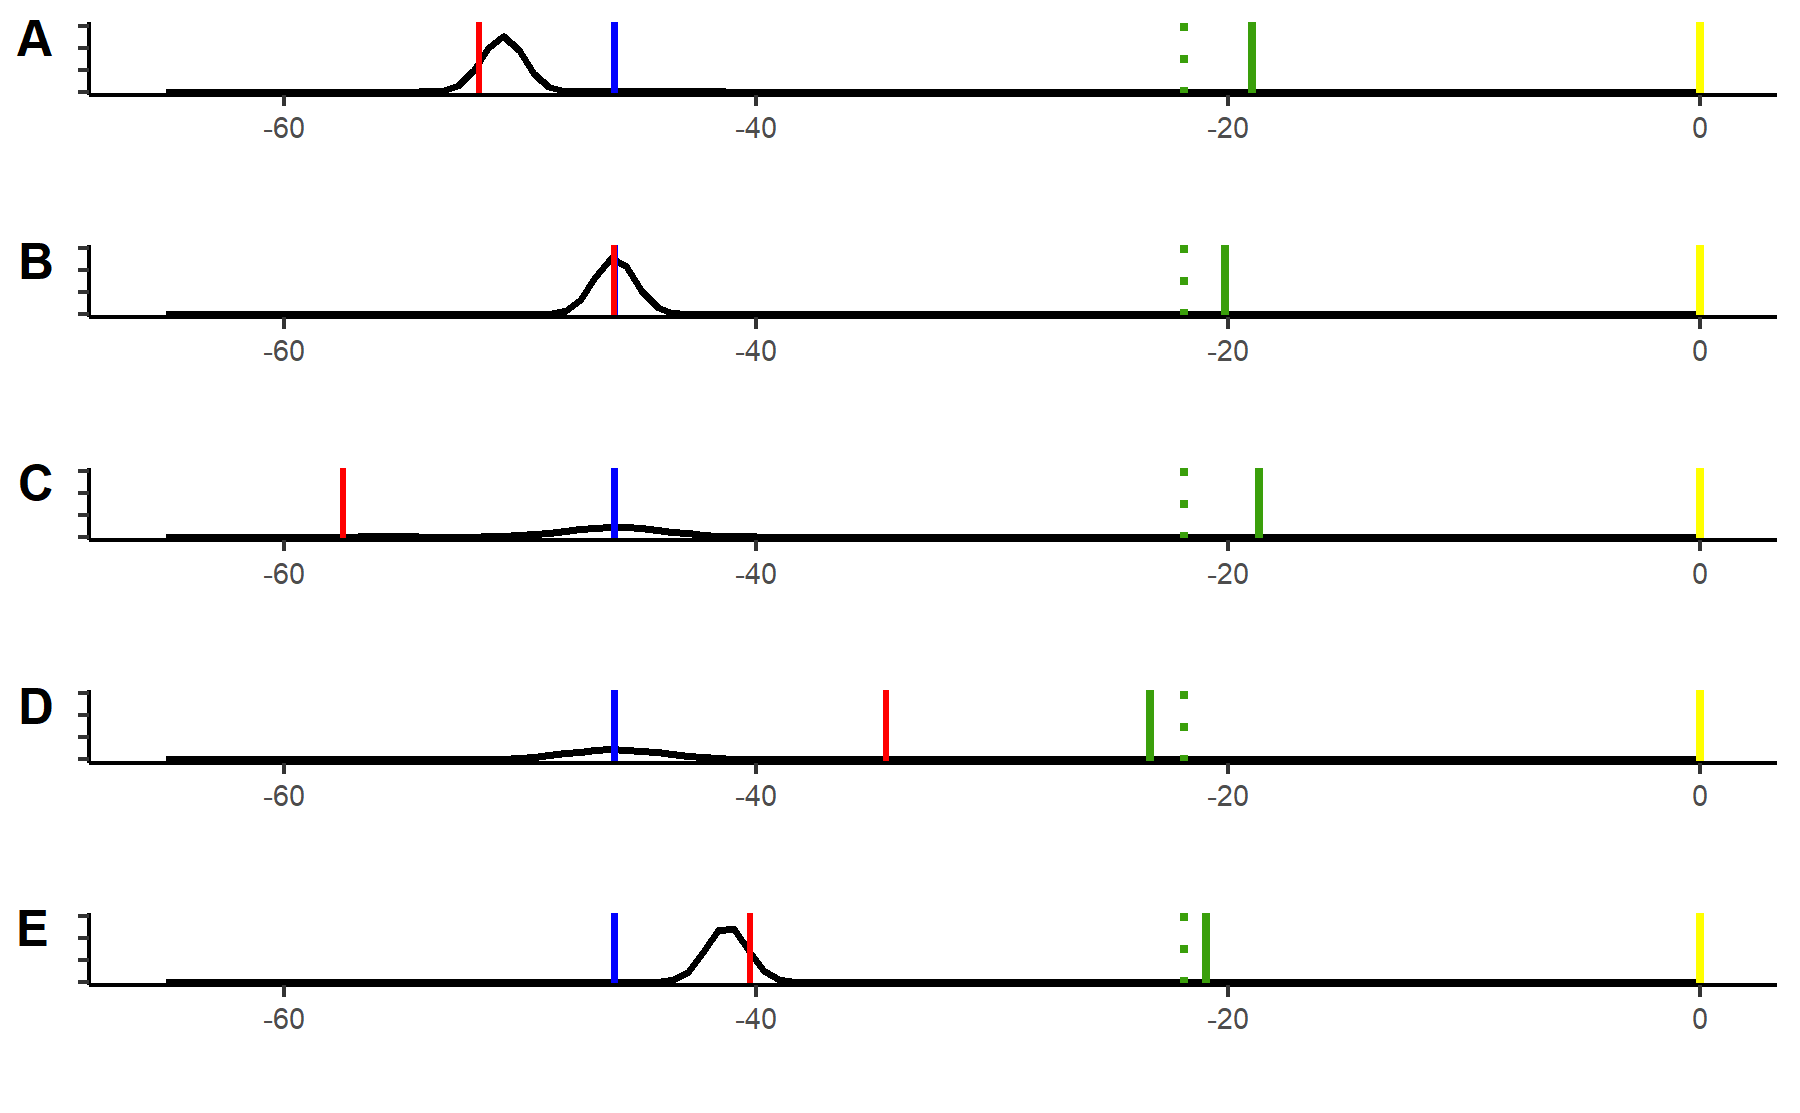
\includegraphics[width=\textwidth, keepaspectratio]{Images/bci_plot2.png}
    \caption{Estimated target location for Target Location = 21.85 cm, for different proximal hand's inferred positions according to the Bayesian Causal Inference Model. The red line indicates position of the visual signal of the proximal hand, while the blue line indicates the position of the proprioceptive signal, that is, the location of the placement of the real hand. The black curve indicates the probability density function denoting the probability of the location of the hand, as postulated by the multi-sensory integration process specified in the Bayesian Causal Inference Model. The mode of the distribution indicates the inferred position of the hand. The green dotted line indicates the veridical position of the reach target, while the solid green line indicates the (average) located estimated by the subjects. The yellow line indicates the initial position of the action hand. Panels A to E are ordered by the increasing proximity of the inferred hand position to the reach target, As seen in the figure, there is no systematic effect of proximity between the target and inferred hand position, and the target location estimation. }
    \label{fig:bci-plot2}
\end{figure}